\documentclass{IEEEoj}
\usepackage{cite}
\usepackage{amsmath,amssymb,amsfonts}
\usepackage{algorithmic}
\usepackage{graphicx,color}
\usepackage{textcomp}
\def\BibTeX{{\rm B\kern-.05em{\sc i\kern-.025em b}\kern-.08em
    T\kern-.1667em\lower.7ex\hbox{E}\kern-.125emX}}
\AtBeginDocument{\definecolor{ojcolor}{cmyk}{0.93,0.59,0.15,0.02}}
\def\OJlogo{\vspace{-14pt}
\includegraphics[height=28pt]{ojits.png}}
\begin{document}
\receiveddate{XX Month, XXXX}
\reviseddate{XX Month, XXXX}
\accepteddate{XX Month, XXXX}
\publisheddate{XX Month, XXXX}
\currentdate{XX Month, XXXX}
\doiinfo{OJITS.2022.1234567}

\title{Preparation of Papers for IEEE OPEN JOURNALS}

\author{FIRST A. AUTHOR\authorrefmark{1}, FELLOW, IEEE, SECOND B.
AUTHOR\authorrefmark{2}, AND THIRD C. AUTHOR,~JR.\authorrefmark{1,2},
MEMBER, IEEE}
\affil{National Institute of Standards and 
Technology, Boulder, CO 80305 USA}
\affil{Department of Physics, Colorado State University, Fort Collins, 
CO 80523 USA}
\corresp{CORRESPONDING AUTHOR: First A. Author (e-mail: author@ boulder.nist.gov).}
\authornote{This work was supported by the Natural Sciences and Engineering Research Council (NSERC) of Canada.}
\markboth{Preparation of Papers for IEEE OPEN JOURNALS}{Author \textit{et al.}}

\begin{abstract}
Air traffic management inefficiencies within terminal maneuvering areas significantly increase environmental and operational costs for the aviation industry. Predicting the additional fuel burn resulting from these inefficiencies remains a complex challenge. In this study, we propose a machine learning framework designed to estimate the excess fuel consumption, recognized internationally as Key Performance Indicator 16, for commercial aircraft arriving at Guarulhos International Airport in Brazil. Our methodology integrates real-world radar trajectories, aircraft performance parameters, and additional transit time metrics into a robust data architecture. We evaluated multiple gradient boosting algorithms to capture the complex relationships between flight trajectory variables and fuel consumption. The comparative analysis reveals that, after hyperparameter optimization, the CatBoost model achieves the most effective balance of predictive performance and generalization, yielding a coefficient of determination of 0.6259 and a root mean squared error of 33.56 kilograms. Furthermore, our feature importance analysis indicates that the predicted transit time within the terminal area is the most critical explanatory variable, emphasizing the direct impact of air traffic congestion and sequencing inefficiencies on fuel burn. Ultimately, the developed approach provides stakeholders with a reliable, data-driven tool for the continuous monitoring of operational efficiency. This framework supports air navigation service providers in optimizing approach procedures, enhancing governance, and aligning operations with global aviation sustainability goals.
\end{abstract}
\begin{IEEEkeywords}
Air traffic management, fuel consumption, gradient boosting, machine learning, terminal maneuvering area.
\end{IEEEkeywords}

%\IEEEspecialpapernotice{(Invited Paper)}

\maketitle

\section{INTRODUCTION}
\label{sec:intro}

The Terminal Maneuvering Area (TMA) is one of the most critical and complex sectors of modern airspace. Operations within this region are characterized by high traffic density, reduced separation minimums, low altitudes, and limited runway capacity. Due to these constraints, air traffic controllers must frequently intervene to maintain safety and sequence arriving aircraft. However, these tactical interventions often disrupt optimal flight profiles. When an aircraft is unable to perform a Continuous Descent Operation (CDO) and is instead forced to level off, enter holding patterns, or follow extended vectoring, it operates at lower, less aerodynamically efficient altitudes. Consequently, these deviations from the optimal trajectory generate a substantial increase in fuel consumption and greenhouse gas emissions.

Given the environmental and economic urgency of modern aviation, managing fuel consumption in the TMA is of utmost importance. The International Civil Aviation Organization (ICAO) has established ambitious global environmental goals, including continuous improvements in fuel efficiency and reducing the environmental footprint of aviation—directly supporting the United Nations' 2030 Agenda for Sustainable Development \cite{doc9750}. Inefficiencies in terminal areas significantly undermine these targets, as operations at lower altitudes burn fuel at much higher rates than during the cruise phase. Therefore, identifying, quantifying, and predicting these inefficiencies is crucial for mitigating the aviation industry's environmental impact and reducing operational costs.

To address these challenges and foster a more efficient global air transport network, ICAO advocates for performance-based management. This framework encourages stakeholders to engage in continuous performance benchmarking, guided at a strategic level by the Global Air Navigation Plan (GANP). In Brazil, the Department of Airspace Control (DECEA), supported by the ATM Performance Commission (CP-ATM), aligns with these global directives by defining operational metrics and conducting post-operational analyses of the Brazilian Airspace Control System (SISCEAB) \cite{mca10022}. By measuring specific outcomes, operators and regulators can share strategic goals and implement data-driven improvements.

Within the context of fuel consumption in the TMA, two Key Performance Indicators (KPIs) defined by the ATM community are particularly relevant: KPI08 (Additional Time in TMA) and KPI16 (Additional Fuel Burn). While KPI08 captures the temporal inefficiencies caused by traffic congestion and sequencing, KPI16 directly quantifies the environmental and economic impact by measuring the excess fuel consumed relative to an unimpeded baseline. Because time and fuel are intrinsically linked in aviation, analyzing both metrics provides a comprehensive view of operational performance. The objective of this paper is to present a machine learning framework capable of estimating the additional fuel consumption (KPI16) for commercial aircraft arriving at Guarulhos International Airport. By utilizing radar trajectory data and EUROCONTROL'S Base of Aircraft Data (BADA) performance parameters, we evaluate multiple gradient boosting techniques to provide a robust predictive tool for continuous performance monitoring \cite{baklacioglu2021fuel}.

The remainder of this paper is organized as follows: Section \ref{sec:background} presents essential background concepts. Section \ref{sec:related_works} reviews related literature and existing performance indicators. Section \ref{sec:proposed_approach} describes the proposed methodology, including data collection, preparation, and machine learning approach. Section \ref{sec:experiments_results} presents the experimental results and analysis. Finally, Section \ref{sec:conclusion} concludes the paper and outlines future work.
\section{EXPERIMENTAL DATA}
\label{sec:experimental_data}
Data was collected from three main sources: surveillance radar data  for civil flights landing in São Paulo/Guarulhos International Airport (ICAO: SBGR) was provided by Operational Data Integrator (ODIN) from Brazilian Airspace Control Institute (ICEA), flight-condition fuel usage for aircraft was extracted from Base of Aircraft Data (BADA) online API \cite{bada_a320} and climate data, including ceiling and visibility, was downloaded from Iowa State University API.

\subsection{ODIN SURVEILLANCE RADAR DATA}
ICEA's ODIN contains operational registries for air traffic all around Brazilian territory, including data from five radar arrays around Brazil: \textit{Amazônico} (located in north), \textit{Brasilia} (center-west), \textit{Recife} (northeast), \textit{Curitiba} (south) and \textit{Atlântico} (oceanic portion). They provide information for latitude, longitude, speed relative to sound, flight level, call sign registration and datetime for registry.

Also, ODIN provides previously calculated KPI08 data \cite{mca10022}, including departure airport, landing airport, call sign, weight class and type for aircraft, landing runway, datetime for entering in Terminal Maneuvering Area (TMA) and KPI08 metric itself \cite{doc9750}. Table \ref{tab:odin_dict} summarizes the specific fields from the ODIN surveillance and KPI08 datasets utilized in this work.

\begin{table}[htbp]
\caption{Data Dictionary for ODIN Surveillance Radar Data}
\label{tab:odin_dict}
\centering
\begin{tabular}{m{0.28\columnwidth} m{0.16\columnwidth} m{0.44\columnwidth}}
\hline
\textbf{Field} & \textbf{Type} & \textbf{Description} \\
\hline
\texttt{call\_sign} & String & Aircraft call sign registration \\
\texttt{adep} & String & Departure airport (ICAO code) \\
\texttt{ades} & String & Landing airport (ICAO code) \\
\texttt{aircraft\_type} & String & Aircraft model (e.g., A320) \\
\texttt{weight\_class} & String & Aircraft weight class (e.g., M, H) \\
\texttt{landing\_runway} & String & Validated landing runway (e.g., 09R) \\
\texttt{tma\_entry\_time} & Datetime & Datetime for entering the TMA \\
\texttt{kpi08} & Float & Calculated KPI08 metric (seconds) \\
\texttt{latitude} & Float & Aircraft latitude position \\
\texttt{longitude} & Float & Aircraft longitude position \\
\texttt{flight\_level} & Integer & Current flight level in hundreds of feet (e.g. 30) \\
\texttt{mach} & Float & Speed relative to sound (Mach) \\
\texttt{timestamp} & Datetime & Radar registry datetime \\
\hline
\end{tabular}
\end{table}

\subsection{BADA EFFICIENCY CHART}
The aircraft efficiency map was computed using the Base of Aircraft Data (BADA) model \cite{bada_a320}, specifically BADA3, which accounts for, among other factors, the aircraft type and flight level in estimating instantaneous fuel consumption. The interface between the model and the study requirements was implemented through the \texttt{pyBADA} support library in Python \cite{pybada}. Table \ref{tab:bada_dict} presents the data dictionary for the BADA performance parameters extracted for our methodology.

\begin{table}[htbp]
\caption{Data Dictionary for BADA Efficiency Chart}
\label{tab:bada_dict}
\centering
\begin{tabular}{m{0.28\columnwidth} m{0.16\columnwidth} m{0.44\columnwidth}}
\hline
\textbf{Field} & \textbf{Type} & \textbf{Description} \\
\hline
\texttt{aircraft} & String & Aircraft model identifier (e.g., A320) \\
\texttt{tas\_ms} & Float & True Airspeed in meters per second \\
\texttt{fl} & Integer & Flight Level in hundreds of feet (e.g., 30) \\
\texttt{fuel\_flow\_kg\_s} & Float & Instantaneous fuel flow in kg/s \\
\hline
\end{tabular}
\end{table}

\subsection{IOWA STATE UNIVERSITY CLIMATE DATA}
Iowa State University provides a public API for daily airport weather observations from around the world. In this article, studies will be focused on SBGR and will include both visibility and ceiling from observation radar. The specific fields retained from this dataset are described in Table \ref{tab:climate_dict}.

\begin{table}[htbp]
\caption{Data Dictionary for Iowa State University Climate Data}
\label{tab:climate_dict}
\centering
\begin{tabular}{m{0.28\columnwidth} m{0.16\columnwidth} m{0.44\columnwidth}}
\hline
\textbf{Field} & \textbf{Type} & \textbf{Description} \\
\hline
\texttt{valid} & Datetime & Observation timestamp (e.g., 2025-01-01 15:00) \\
\texttt{station} & String & Weather station ICAO code (e.g., SBSP) \\
\texttt{vsby} & Float & Visibility measurement (in miles) \\
\texttt{ceiling\_ft} & Float & Cloud ceiling height (in feet) \\
\hline
\end{tabular}
\end{table}
\section{DATA PREPARATION AND HANDLING}

The data for this paper were organized with possible scalability in mind. The source of the dataset is the Operational Data Integrator (ODIN) PostgreSQL database maintained by Brazilian Airspace Control Institute (ICEA); the records collected range from January 1 to December 31, 2025. Extraction was performed using Python scripts that produced Parquet files optimized for analytical workloads and stored locally. Subsequent data transformation employed DuckDB as the query engine, with transformations orchestrated through data build tool (dbt), forming a Medallion Architecture data pipeline \cite{databricks_medallion, saha_dataeng}. The resulting datasets were again exported as Parquet files for downstream analysis in Python. The stack used for this work is schematized on Figure \ref{fig:odin-etl-simplified}.

\begin{figure}[htbp]
    \centering
    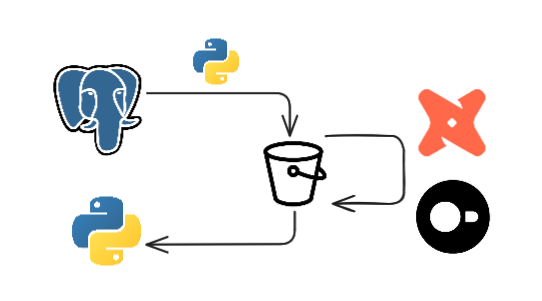
\includegraphics[width=1\linewidth]{images/odin-etl-simplified.png}
    \caption{Simplified schematics for the stack used in this work.}
    \label{fig:odin-etl-simplified}
\end{figure}

\subsection{FEATURE ENGINEERING}

To enhance the analytical value of the flight data, a series of feature engineering transformations were applied using DuckDB and subsequently orchestrated and documented through dbt. We focused on creating features that better represented flight behavior, airspace congestion, and operational context.

The data transformations were structured across multiple SQL models to progressively build the final dataset:

\begin{itemize}
    \item \textbf{Trajectory Tracking and Elapsed Time:} The radar trajectory points were bounded between the time the aircraft crossed the TMA cylinder (\textit{c\_time}) and the actual landing time (\textit{aldt}). For each flight level (FL) recorded, the time difference between consecutive radar pings was calculated to establish the \textit{elapsed} time spent at each altitude.
    
    \item \textbf{Fuel Consumption Estimation:} The \textit{elapsed} time per flight level was multiplied by the aircraft's specific average fuel flow rate (kg/s) obtained from the BADA performance tables \cite{bada_a320, pybada}. The sum of these values across all flight levels yielded the total fuel consumption in the terminal area (\textit{consumption\_kg}).
    
    \item \textbf{Airspace Congestion Tracking:} To represent the dynamic traffic density, an event-based running sum was implemented. Every \textit{c\_time} was treated as an entry (+1) and every \textit{aldt} as an exit (-1). Using SQL window functions over the chronological timeline, we calculated the exact number of aircraft present in the TMA at any given moment (\textit{nr\_aircraft\_in\_tma}).
    
    \item \textbf{Rolling Predictive Metrics:} A moving average for the time spent in the TMA (\textit{transit\_tma\_predicted}) was created to mimic the expected transit time given recent conditions. This was calculated over a 1-hour rolling window preceding the flight, partitioned by the validated runway (\textit{drwy\_validado}) and the entry sector (\textit{setor}).
    
    \item \textbf{Baseline Efficiency and Target Variable:} To define a standard for efficient operations, we calculated the 20th percentile of fuel consumption (\textit{consumption\_20p}) partitioned by departure airport (\textit{adep}), aircraft type, and landing runway. Finally, the main target variable for this study, \textit{kpi16}, was computed as the difference between the actual fuel consumption (\textit{consumption\_kg}) and this 20th percentile baseline.
    
    \item \textbf{Temporal and Environmental Variables:} Datetime fields were decomposed into specific categories (\textit{day}, \textit{month}, \textit{hour}, and \textit{day of week}) to capture seasonal and daily patterns. Additionally, weather information from the METAR database (Iowa State University public API) was joined by the hour, incorporating horizontal visibility and cloud ceiling to assess their impact on flight holding and routing.
\end{itemize}

These transformations—ranging from chronological event tracking to percentile-based baselining—were carefully designed to expose underlying trends, airspace bottlenecks, and correlations within the flight data, paving the way for sophisticated machine learning investigations. Furthermore, adopting structured data modeling approaches (e.g., Medallion architecture) ensures scalability when applying these pipelines to massive Apache Spark or distributed SQL environments \cite{databricks_medallion, saha_dataeng}.
% \input{chapters/units}
% \input{chapters/common_mistakes}
% \input{chapters/guidelines}
% \section{CONCLUSION}

In this paper, we successfully developed and validated a machine learning framework to estimate the additional fuel consumption (KPI16) during the terminal maneuvering area (TMA) operations at Guarulhos International Airport. By integrating real-world radar trajectories, BADA performance parameters, and existing operational metrics (such as KPI08) into a scalable data architecture, we created a robust and reproducible analytical pipeline.

The comparative analysis of gradient boosting algorithms demonstrated that the LightGBM model achieved the most effective balance of predictive performance and generalization, with an $R^2$ of 0.64 and a mean absolute error of 17.85 kg. Furthermore, our feature importance analysis highlighted that the predicted transit time within the TMA was the most significant explanatory variable. This finding underscores the direct impact of air traffic congestion and sequencing inefficiencies on both environmental and operational costs.

The resulting methodology provides a reliable tool for the continuous monitoring of operational efficiency, aligning with international sustainability goals and the performance-based management advocated by ICAO. Future work will focus on expanding the scope of the model to encompass other aircraft families and major airports. Additionally, we plan to incorporate real-time meteorological conditions and air traffic flow management (ATFM) data to further enhance predictive accuracy, and to deploy the model within institutional dashboards for automated, near real-time KPI monitoring.
% \section*{APPENDIX}
Appendixes, if needed, appear before the acknowledgment.
% \input{chapters/acknowledgment}
% \section*{REFERENCES AND FOOTNOTES}
\subsection{REFERENCES}
References need not be cited in text. When they are, they appear on the 
line, in square brackets, inside the punctuation. Multiple references are 
each numbered with separate brackets. When citing a section in a book, 
please give the relevant page numbers. In text, refer simply to the 
reference number. Do not use ``Ref.'' or ``reference'' except at the 
beginning of a sentence: ``Reference [3] shows \textellipsis .'' Please do not use 
automatic endnotes in \textit{Word}, rather, type the reference list at the end of the 
paper using the ``References'' style.

Reference numbers are set flush left and form a column of their own, hanging 
out beyond the body of the reference. The reference numbers are on the line, 
enclosed in square brackets. In all references, the given name of the author 
or editor is abbreviated to the initial only and precedes the last name. Use 
them all; use \textit{et al}. only if names are not given. Use commas around Jr., Sr., and 
III in names. Abbreviate conference titles. When citing IEEE transactions, 
provide the issue number, page range, volume number, year, and/or month if 
available. When referencing a patent, provide the day and the month of 
issue, or application. References may not include all information; please 
obtain and include relevant information. Do not combine references. There 
must be only one reference with each number. If there is a URL included with 
the print reference, it can be included at the end of the reference. 

Other than books, capitalize only the first word in a paper title, except 
for proper nouns and element symbols. For papers published in translation 
journals, please give the English citation first, followed by the original 
foreign-language citation See the end of this document for formats and 
examples of common references. For a complete discussion of references and 
their formats, see the IEEE style manual at www.ieee.org/authortools.


\subsection{FOOTNOTES}
Number footnotes separately in superscripts (Insert\textbar 
Footnote).\footnote{It is recommended that footnotes be avoided (except for 
the unnumbered footnote with the receipt date on the first page). Instead, 
try to integrate the footnote information into the text.} Place the actual 
footnote at the bottom of the column in which it is cited; do not put 
footnotes in the reference list (endnotes). Use letters for table footnotes 
(see Table I). 

% \input{chapters/submission}
% \section{IEEE PUBLISHING POLICY}
The general IEEE policy requires that authors should only submit original 
work that has neither appeared elsewhere for publication, nor is under 
review for another refereed publication. The submitting author must disclose 
all prior publication(s) and current submissions when submitting a 
manuscript. Do not publish ``preliminary'' data or results. The submitting 
author is responsible for obtaining agreement of all coauthors and any 
consent required from employers or sponsors before submitting an article. 
The IEEE Open Journals Department strongly discourages courtesy authorship; 
it is the obligation of the authors to cite only relevant prior work.

The IEEE Open Journals Department does not publish conference records or 
proceedings, but can publish articles related to conferences that have 
undergone rigorous peer review. Minimally, two reviews are required for 
every article submitted for peer review.
% \input{chapters/publication_principles}
% \section*{REFERENCES}

\def\refname{\vadjust{\vspace*{-1em}}} %Please don't do this in a real paper.

\subsubsection*{Basic format for books:}

\begin{thebibliography}{00}
\bibitem{b1} J. K. Author, ``Title of chapter in the book,'' in \textit{Title of His Published Book, x}th ed. City of Publisher,
(only U.S. State), Country: Abbrev. of Publisher, year, ch. x, sec. x, pp.
\textit{xxx--xxx.}
\end{thebibliography}

\subsubsection*{Examples:}

\begin{thebibliography}{00}
\bibitem{b2} G. O. Young, ``Synthetic structure of industrial
plastics,'' in \emph{Plastics}, 2nd ed., vol. 3, J. Peters, Ed. New York, NY, USA: McGraw-Hill, 1964, pp. 15--64.
\bibitem{b3} W.-K. Chen, \emph{Linear Networks and Systems}. Belmont, CA, USA: Wadsworth, 1993, pp. 123--135.
\end{thebibliography}

\subsubsection*{Basic format for periodicals:}

\begin{thebibliography}{00}
\bibitem{b4} J. K. Author, ``Name of paper,'' \textit{Abbrev. Title of Periodical}, vol. x, no. x, pp. xxx-xxx, Abbrev. Month, year, DOI.
10.1109.\textit{XXX}.123456.
\end{thebibliography}

\subsubsection*{Examples:}

\begin{thebibliography}{00}
\bibitem{b5} J. U. Duncombe, ``Infrared navigation---Part I: An
assessment of feasibility,'' \emph{IEEE Trans. Electron Devices}, vol. ED-11, no. 1, pp. 34--39, Jan. 1959, 10.1109/TED.2016.2628402.
\bibitem{b6} E. P. Wigner, ``Theory of traveling-wave optical laser,'' 
\emph{Phys. Rev.}, vol. 134, pp. A635--A646, Dec. 1965.
\bibitem{b7} E. H. Miller, ``A note on reflector arrays,'' \emph{IEEE
Trans. Antennas Propagat.}, to be published.
\bibitem{b8} H. Qin, Y. Cui, Z. Wu, Q. Chen and D. Xing, "Real-Time
Thermoacoustic Imaging-Guidance for Breast Tumor Resection," \emph{IEEE Photonics Journal}, vol. 12, no. 3, pp. 1--7, June 2020, Art no. 3700207.
\end{thebibliography}

\subsubsection*{Basic format for reports:}

\begin{thebibliography}{00}
\bibitem{b9} J. K. Author, ``Title of report,'' Abbrev. Name of Co., City of Co., Abbrev.
State, Country, Rep. {xxx}, year.
\end{thebibliography}

\subsubsection*{Examples:}

\begin{thebibliography}{00}
\bibitem{b10} E. E. Reber, R. L. Michell, and C. J. Carter, ``Oxygen absorption in the earth's atmosphere,'' Aerospace Corp., Los Angeles, CA, USA, Tech. Rep. TR-0200 (4230-46)-3, Nov. 1988.
\bibitem{b11} J. H. Davis and J. R. Cogdell, ``Calibration program for the 16-foot antenna,'' Elect. Eng. Res. Lab., Univ. Texas, Austin, TX, USA, Tech. Memo. NGL-006-69-3, Nov. 15, 1987.
\end{thebibliography}

\subsubsection*{Basic format for handbooks:}

\begin{thebibliography}{00}
\bibitem{b12} \textit{Name of Manual/Handbook}, x ed., Abbrev. Name of Co., City of Co., Abbrev. State, Country, year, pp.
\textit{xxx-xxx.}
\end{thebibliography}

\subsubsection*{Examples:}

\begin{thebibliography}{00}
\bibitem{b13} \textit{Transmission Systems for Communications}, 3rd ed., Western Electric Co., Winston-Salem, NC, USA, 1985, pp. 44--60.
\bibitem{b14} \textit{Motorola Semiconductor Data Manual}, Motorola Semiconductor Products Inc., Phoenix, AZ, USA, 1989.
\end{thebibliography}

\subsubsection*{Basic format for books (when available online): }

\begin{thebibliography}{00}
\bibitem{b15} J. K. Author, ``Title of chapter in the book,'' in \textit{Title of Published Book}, xth ed. City of
Publisher, State, Country: Abbrev. of Publisher, year, ch. x, sec. x, pp.
\textit{xxx--xxx}. [Online]. Available: \underline {http://www.web.com}. Accessed on: Month
Day, Year.
\end{thebibliography}

\subsubsection*{Examples:}

\begin{thebibliography}{00}
\bibitem{b16} G. O. Young, ``Synthetic structure of industrial
plastics,'' in \emph{Plastics}, vol. 3, Polymers of Hexadromicon, J.
Peters, Ed., 2nd ed. New York, NY, USA: McGraw-Hill, 1964, pp. 15--64.
[Online]. Available: \underline{http://www.bookref.com}. Accessed on: April 25, 2020.
\bibitem{b17} \textit{The Founders' Constitution}, Philip B. Kurland and Ralph Lerner, eds., Chicago, IL, USA: Univ. Chicago Press, 1987. [Online]. Available: \underline {http://press-pubs.uchicago.edu/founders/}. Accessed on: April 25, 2020.
\bibitem{b18} \emph{The Terahertz Wave eBook}. ZOmega Terahertz
Corp., 2014. [Online]. Available: \underline{http://dl.z-thz.com/eBook/zomega\_ebook\_pdf\_1206\_sr.pdf}. Accessed on: May 19, 2014.
\bibitem{b19} Philip B. Kurland and Ralph Lerner, eds., \textit{The
Founders' Constitution. }Chicago, IL, USA: Univ. of Chicago Press, 1987, [Online] Available: \emph{http://press-pubs.uchicago.edu/founders/}. Accessed on: Feb. 28, 2010.
\end{thebibliography}

\subsubsection*{Basic format for conference proceedings (published):}

\begin{thebibliography}{00}
\bibitem{b20} J. K. Author, ``Title of paper,'' in \textit{Abbreviated Name of Conf.}, City of Conf., Abbrev. State (if
given), Country, year, pp. \textit{xxxxxx.}
\end{thebibliography}

\subsubsection*{Example:}

\begin{thebibliography}{00}
\bibitem{b21} D. B. Payne and J. R. Stern, ``Wavelength-switched
passively coupled single-mode optical network,'' in \textit{Proc. IOOC-ECOC, }Boston, MA, USA, 1985,~pp.~585--590.
\end{thebibliography}

\subsubsection*{Basic format for papers presented at conferences when available online: }

\begin{thebibliography}{00}
\bibitem{b22} J.K. Author. (year, month). Title. presented at abbrev. conference title.
[Type of Medium]. Available: \underline{site/path/file}. Accessed on: Month Day, Year.
\end{thebibliography}

\subsubsection*{Example:}

\begin{thebibliography}{00}
\bibitem{b23} PROCESS Corporation, Boston, MA, USA. Intranets: Internet technologies deployed behind the firewall for corporate productivity. Presented at INET96 Annual Meeting. [Online]. Available: \underline {http://home.process.com/Intranets/wp2.htp}. Accessed on: April 25, 2020.
\end{thebibliography}

\subsubsection*{Basic format for reports and handbooks (when available online): }

\begin{thebibliography}{00}
\bibitem{b24} J. K. Author. ``Title of report,'' Company. City, State, Country. Rep. no.,
(optional: vol./issue), Date. [Online] Available:
\underline{site/path/file}. Accessed
on: Month Day, Year.
\end{thebibliography}

\subsubsection*{Examples:}

\begin{thebibliography}{00}
\bibitem{b25} R. J. Hijmans and J. van Etten, ``Raster: Geographic analysis and modeling with raster data,'' R Package Version 2.0-12, Jan. 12, 2012. [Online]. Available: \underline {http://CRAN.R-project.org/package=raster}. Accessed on: April 25, 2020.
\bibitem{b26} Teralyzer. Lytera UG, Kirchhain, Germany [Online]. Available: \emph{http://www.lytera.de/Terahertz\_THz\_Spectroscopy.php?id=home}, Accessed on: Jun. 5, 2014
\end{thebibliography}

\subsubsection*{Basic format for computer programs and electronic documents (when available online): }

\begin{thebibliography}{00}
\bibitem{b27} Legislative body. Number of Congress, Session. (year, month day). \textit{Number of bill or resolution}, \textit{Title}. [Type
of medium]. Available: \underline{site/path/file}
\end{thebibliography}

{\bfseries\itshape NOTE:} ISO recommends that capitalization follow the
accepted practice for the language or script in which the information is
given.

\subsubsection*{Example:}

\begin{thebibliography}{00}
\bibitem{b28} U.S. House. 102nd Congress, 1st Session. (1991, Jan. 11). \textit{H. Con. Res. 1, Sense of the Congress on Approval of Military Action}. [Online]. Available: LEXIS Library: GENFED File: BILLS
\end{thebibliography}

\subsubsection*{Basic format for patents (when available online):}

\begin{thebibliography}{00}
\bibitem{b29} Name of the invention, by inventor's name. (year, month day). Patent Number [Type
of medium]. Available: \underline{site/path/file}
\end{thebibliography}

\subsubsection*{Example:}

\begin{thebibliography}{00}
\bibitem{b30} Musical toothbrush with mirror, by L.M.R. Brooks. (1992, May 19). Patent D 326 189 [Online]. Available: NEXIS Library: LEXPAT File: DES
\end{thebibliography}

\subsubsection*{Example for papers presented at conferences (unpublished):}

\begin{thebibliography}{00}
\bibitem{b31} D. Ebehard and E. Voges, ``Digital single sideband
detection for interferometric sensors,'' presented at the \textit{2nd Int. Conf. Optical Fiber Sensors,} Stuttgart, Germany, Jan. 2--5, 1984.
\end{thebibliography}

\subsubsection*{Basic format for patents:}

\begin{thebibliography}{00}
\bibitem{b32} J. K. Author, ``Title of patent,'' U.S. Patent {x xxx xxx}, Abbrev. Month, day, year.
\end{thebibliography}

\subsubsection*{Example:}

\begin{thebibliography}{00}
\bibitem{b33} G. Brandli and M. Dick, ``Alternating current fed power supply,'' U.S. Patent 4 084 217, Nov. 4, 1978.
\end{thebibliography}

\subsubsection*{Basic format for theses (M.S.) and dissertations (Ph.D.):}

\begin{thebibliography}{00}
\bibitem{b34} J. K. Author, ``Title of thesis,'' M.S. thesis, Abbrev. Dept., Abbrev.
Univ., City of Univ., Abbrev. State, year. p. nnn.
\bibitem{b35} J. K. Author, ``Title of dissertation,'' Ph.D. dissertation, Abbrev.
Dept., Abbrev. Univ., City of Univ., Abbrev. State, year. p. nnn.
\end{thebibliography}

\subsubsection*{Examples:}

\begin{thebibliography}{00}
\bibitem{b36} J. O. Williams, ``Narrow-band analyzer,'' Ph.D. dissertation, Dept. Elect. Eng., Harvard Univ., Cambridge, MA, USA, 1993. p. 50.
\bibitem{b37} N. Kawasaki, ``Parametric study of thermal and chemical nonequilibrium nozzle flow,'' M.S. thesis, Dept. Electron. Eng., Osaka Univ., Osaka, Japan, 1993. p. 30.
\end{thebibliography}

\subsubsection*{Basic format for the most common types of unpublished references:}

\begin{thebibliography}{00}
\bibitem{b38} J. K. Author, private communication, Abbrev. Month, year.
\bibitem{b39} J. K. Author, ``Title of paper,'' unpublished.
\bibitem{b40} J. K. Author, ``Title of paper,'' to be published.
\end{thebibliography}

\subsubsection*{Examples:}

\begin{thebibliography}{00}
\bibitem{b41} A. Harrison, private communication, May 1995.
\bibitem{b42} B. Smith, ``An approach to graphs of linear forms,'' unpublished.
\bibitem{b43} A. Brahms, ``Representation error for real numbers in binary computer arithmetic,'' IEEE Computer Group Repository, Paper R-67-85.
\end{thebibliography}

\subsubsection*{Basic formats for standards:}

\begin{thebibliography}{00}
\bibitem{b44} \textit{Title of Standard}, Standard number, date.
\bibitem{b45} \textit{Title of Standard}, Standard number, Corporate author, location, date.
\end{thebibliography}

\subsubsection*{Examples:}

\begin{thebibliography}{00}
\bibitem{b46} \emph{IEEE Criteria for Class IE Electric Systems}, IEEE Standard 308, 1969.
\bibitem{b47} \emph{Letter Symbols for Quantities}, ANSI Standard Y10.5-1968.
\end{thebibliography}

\subsubsection*{Article number in~reference examples:}

\begin{thebibliography}{00}
\bibitem{b48} R. Fardel, M. Nagel, F. Nuesch, T. Lippert, and A. Wokaun, ``Fabrication of organic light emitting diode pixels by laser-assisted forward transfer,'' \textit{Appl. Phys. Lett.}, vol. 91, no. 6, Aug. 2007, Art. no. 061103.
\bibitem{b49} J. Zhang and N. Tansu, ``Optical gain and laser characteristics of InGaN quantum wells on ternary InGaN substrates,'' \textit{IEEE Photon. J.}, vol. 5, no. 2, Apr. 2013, Art. no. 2600111
\end{thebibliography}

\subsubsection*{Example when using et al.:}

\begin{thebibliography}{00}
\bibitem{b50} S. Azodolmolky, Jordi Perell\'{o}, Marianna Angelou, Fernando Agraz, Luis Velasco, Salvatore Spadaro,~\textit{et al.}, Experimental demonstration of an impairment aware network planning and operation tool for transparent/translucent optical networks,''~\textit{J. Lightwave. Technol.}, vol. 29, no. 4, pp. 439--448, Sep. 2011.
\end{thebibliography}

\begin{IEEEbiography}[{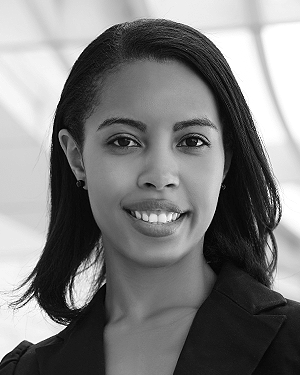
\includegraphics[width=1in,height=1.25in,clip,keepaspectratio]{a1.png}}]{FIRST
A. AUTHOR } (Fellow, IEEE) and all authors may include 
biographies. Biographies are often not included in conference-related
papers. This author became a Member (M) of IEEE in 1976, a Senior
Member (SM) in 1981, and a Fellow (F) in 1987. The first paragraph may
contain a place and/or date of birth (list place, then date). Next,
the author's educational background is listed. The degrees should be
listed with type of degree in what field, which institution, city,
state, and country, and year the degree was earned. The author's major
field of study should be lower-cased. 

The second paragraph uses the pronoun of the person (he or she) and not the 
author's last name. It lists military and work experience, including summer 
and fellowship jobs. Job titles are capitalized. The current job must have a 
location; previous positions may be listed 
without one. Information concerning previous publications may be included. 
Try not to list more than three books or published articles. The format for 
listing publishers of a book within the biography is: title of book 
(publisher name, year) similar to a reference. Current and previous research 
interests end the paragraph. The third paragraph begins with the author's 
title and last name (e.g., Dr.\ Smith, Prof.\ Jones, Mr.\ Kajor, Ms.\ Hunter). 
List any memberships in professional societies other than the IEEE. Finally, 
list any awards and work for IEEE committees and publications. If a 
photograph is provided, it should be of good quality, and 
professional-looking. Following are two examples of an author's biography.
\end{IEEEbiography}

\begin{IEEEbiography}[{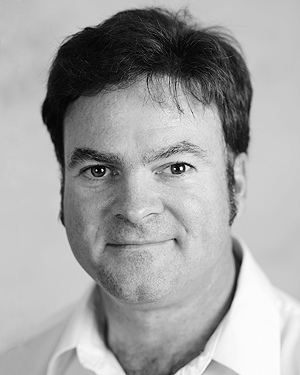
\includegraphics[width=1in,height=1.25in,clip,keepaspectratio]{a2.png}}]{SECOND
B. AUTHOR } was born in Greenwich Village, New York, NY, USA in 
1977. He received the B.S. and M.S. degrees in aerospace engineering from 
the University of Virginia, Charlottesville, in 2001 and the Ph.D. degree in 
mechanical engineering from Drexel University, Philadelphia, PA, in 2008.

From 2001 to 2004, he was a Research Assistant with the Princeton Plasma 
Physics Laboratory. Since 2009, he has been an Assistant Professor with the 
Mechanical Engineering Department, Texas A{\&}M University, College Station. 
He is the author of three books, more than 150 articles, and more than 70 
inventions. His research interests include high-pressure and high-density 
nonthermal plasma discharge processes and applications, microscale plasma 
discharges, discharges in liquids, spectroscopic diagnostics, plasma 
propulsion, and innovation plasma applications. He is an Associate Editor of 
the journal \emph{Earth, Moon, Planets}, and holds two patents. 

Dr. Author was a recipient of the International Association of Geomagnetism 
and Aeronomy Young Scientist Award for Excellence in 2008, and the IEEE 
Electromagnetic Compatibility Society Best Symposium Paper Award in 2011. 
\end{IEEEbiography}

\begin{IEEEbiography}[{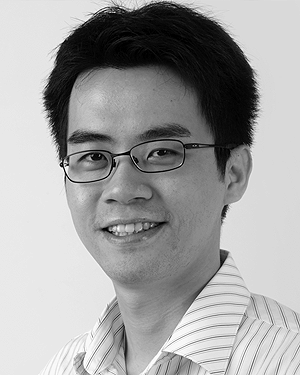
\includegraphics[width=1in,height=1.25in,clip,keepaspectratio]{a3.png}}]{THIRD
C. AUTHOR,~JR. } (Member, IEEE) received the B.S. degree in mechanical 
engineering from National Chung Cheng University, Chiayi, Taiwan, in 2004 
and the M.S. degree in mechanical engineering from National Tsing Hua 
University, Hsinchu, Taiwan, in 2006. He is currently pursuing the Ph.D. 
degree in mechanical engineering at Texas A{\&}M University, College 
Station, TX, USA.

From 2008 to 2009, he was a Research Assistant with the Institute of 
Physics, Academia Sinica, Tapei, Taiwan. His research interest includes the 
development of surface processing and biological/medical treatment 
techniques using nonthermal atmospheric pressure plasmas, fundamental study 
of plasma sources, and fabrication of micro- or nanostructured surfaces. 

Mr. Author's awards and honors include the Frew Fellowship (Australian 
Academy of Science), the I. I. Rabi Prize (APS), the European Frequency and 
Time Forum Award, the Carl Zeiss Research Award, the William F. Meggers 
Award and the Adolph Lomb Medal (OSA).
\end{IEEEbiography}

\end{document}
